\section{Tickets}
In the HOPR protocol, nodes that have staked funds within a payment channel can issue tickets that are used for payment to other nodes. 
Tickets are used for probabilistic payments; every ticket is bound to a specific payment channel and cannot be spent elsewhere. 
They are redeemable at most once and they lose their value when the channel is closed or when the commitment is reset. 
\subsection{Ticket issuance}
A ticket can be issued once two nodes have established a payment channel with each other which means that at least one of them has locked HOPR tokens.
\newline The ticket issuer A (A could also be the packet creator) selects the winning probability of the ticket and the relay fee to use and sets amount to:
$$\delta:=\dfrac{L*F}{P_w}$$
where $\delta$ is the amount of HOPR tokens set in the ticket, $L$ is the path length, $F$ is the relay fee and $P_w$ is the winning probability.
\\~\\The issuer $(A)$ issues a ticket for the next downstream node, 
the challenge is given together with the routing information by the packet. 
\\$(A)$ does not know whether the ticket is a win or not.
\\$(A)$ sets content of a ticket to: $$t=(R, C, \alpha_c, \delta, P_w, \zeta, I)$$ 
where $R$ is the recipient, $C$ is the challenge, $\alpha_c$ is the account.counter, $\zeta$ is the channel.iteration and $I$ is the index.
\\$(A)$ then signs the ticket with its private key and sends $T:= (t, Sig_I(t))$ to the recipient together with a mixnet packet.
\\The data for a ticket is signed by the issuer, and a ticket is the data followed by the signature: $$T:=(T_D,Sig_{I}(T_D))$$ where 
    $$T_D:=(\delta,P_w,R,I,C,\zeta,c_{Id},tag,V)$$
 \begin{figure}[H]
    \centering
    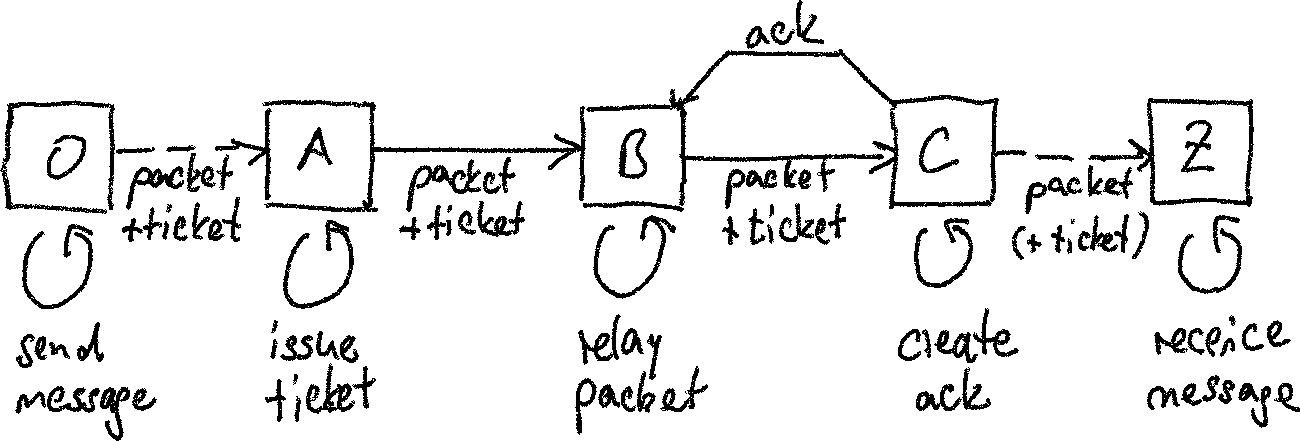
\includegraphics[width=10cm,height=10cm,keepaspectratio]{../whitepaper/images/ticket_workflow.png}
    \caption{Ticket workflow}
    \label{fig:Ticket worklow}
\end{figure}

\subsubsection{Challenge}
$(A)$ creates a shared secret $s_i$ with all the relay nodes in the channel (B-C-D-Z) by using an offline version of the Diffie-Hellman key exchange.
\newline The shared secret $s_i$ is used as a seed for a PRG (Pseudo Random Generator) to create secret shares $s_i,s_i'$ for each node along the route. 
Relayers compute $s_i$ and get $s_{i+1}'$ from the next downstream node. 
\newline The sender $(A)$ creates $challenge_i:=(s_i+s_{i+1}')*G$ and a hint for B,C,D,Z (let’s suppose these are the relay nodes and $Z$ will be the final destination) a “hint” how the promised value $s_C',s_D',s_Z'$ is going to look like. 
The value “hint” is computed as $hint_i:=s_{i+1}'*G$ 


\subsection{Ticket validation}
Tickets are received together with packets which means that the recipient and the next downstream node share a secret $s$ whose key shares $s_i$ and $s_{i+1}$ are derivable by those nodes.
\newline Once $(A)$ receives $s_{i+1}^{(1)}$ from (B) by the secret sharing, it can compute $response:=s_i^{(0)}+s_{i+1}^{(1)}$ such that it verifies  
$$response*G=ticket.challenge$$
Once the recipient transforms the packet, it is able to compute $s_i$. The recipient is now also able to extract the routing information from the packet. 
This includes a hint to the value $s_{i+1}$ given as $hint_i:=s_{i+1}*G$.
\\The unacknowledged ticket is stored in the database under the $hint$ to the promised value to make sure that the acknowledgement can be afterwards linked to the unacknowledged ticket.
\newline Together with $s_i$, the node can verify that $$ticket.challenge=s_i*G+hint_i$$ with $$s_i*G+hint=s_i*G+s_{i+1}*G=(s_i+s_{i+1})*G$$ 
This allows the recipient to verify that the promised value $s_{i+1}$ indeed leads to a solution of the challenge given in the ticket. 
If this is not the case, then the node should drop the packet.
\newline Without this check, the sender is able to intentionally create falsy challenges that lead to unredeemable tickets.


\subsection{Ticket redemption}


In order to unlock the ticket, the node stores it within its database until it receives an acknowledgement containing $s_{i+1}$ from the next downstream node. 
The challenge can be computed from acknowledgement as $challenge:=ack*G$.
\newline Once it receives an acknowledgement, it checks whether it stores an unacknowledged ticket for the received acknowledgement. 
If this is not the case, the node should drop the acknowledgement.  
\newline The node then computes the response to the challenge given in the ticket as $$response:=(s_i+s_{i+1})*G$$
Additionally, the node retrieves the opening value open to the current on-chain commitment and checks whether response, open leads to a winning ticket. 
This is the case if $$H( ticketHash, response, open ) <P_w$$ where $$ticketHash:=H(T_D)$$
If this is not the case, the node should drop the ticket. 
The final recipient of the packet does not receive a ticket because message reception is not incentivized by the HOPR protocol.
\newline The node checks whether the information gained from the packet transformation is sufficient to fulfill the given challenge sent along with the ticket. It then replies with an acknowledgement that includes a response to the challenge.
\\ The node also checks the following:
\begin{itemize}
    \item The signature of the ticket issuer is valid: $$ecrecover(Sig_{response}(0))=address(T_D.challenge)$$
    \item The ticket has been already spent (replay protection): $$channel.index <T_D.index$$
    \item Channel exists and is open.
    \item Channel balance towards the ticket recipient is sufficient to cover the costs for the ticket.
    \item Ticket index is strictly greater than the current value in the smart contract (reorder protection). This is valid because redeeming a $ticket$ with $index=n$ requires $index < n+1$ and sets $index := n+1$. So the new index becomes greater than $n$.


\end{itemize}  








